\documentclass[conference]{IEEEtran}
\IEEEoverridecommandlockouts
% The preceding line is only needed to identify funding in the first footnote. If that is unneeded, please comment it out.
\usepackage{cite}
\usepackage{amsmath,amssymb,amsfonts}
\usepackage{algorithmic}
\usepackage{graphicx}
\usepackage{textcomp}
\usepackage{xcolor}
\usepackage{tikz}
\usetikzlibrary{arrows.meta, positioning}
\def\BibTeX{{\rm B\kern-.05em{\sc i\kern-.025em b}\kern-.08em
    T\kern-.1667em\lower.7ex\hbox{E}\kern-.125emX}}
% The following packages can be found on http:\\www.ctan.org
\usepackage{bm}
\newcommand{\uvec}[1]{\boldsymbol{\hat{\textbf{#1}}}}
%\usepackage{epsfig} % for postscript graphics files
%\usepackage{mathptmx} % assumes new font selection scheme installed
%\usepackage{times} % assumes new font selection scheme installed
%\usepackage{amsmath} % assumes amsmath package installed
%\usepackage{amssymb}  % assumes amsmath package installed

\usepackage{listings}
\usepackage[T1]{fontenc} % optional but nice for tt fonts
\usepackage{float}

\lstset{
  basicstyle=\ttfamily\footnotesize,
  breaklines=true,
  breakatwhitespace=true,
  columns=fullflexible,
  keepspaces=true,
}


% ============================================================================
% Title and Authors (translated from main.tex)
% ============================================================================

\title{Predicting Online Shoppers’ Purchasing Intention}

\author{%
\IEEEauthorblockN{Anthony Stefanuto}
\IEEEauthorblockA{Computer Science\\
Western University}
\and
\IEEEauthorblockN{Luke Jang}
\IEEEauthorblockA{Computer Science\\
Western University}
\and
\IEEEauthorblockN{Aimee Tang}
\IEEEauthorblockA{Statistics\\
Western University}
\and
\IEEEauthorblockN{Nicol Elias}
\IEEEauthorblockA{Statistics\\
Western University}
}

\begin{document}

\maketitle

%%%%%%%%%%%%%%%%%%%%%%%%%%%%%%%%%%%%%%%%%%%%%%%%%%%%%%%%%%%%%%%%%%%%%%%%%%%%%%%%
\begin{abstract} 
How to conceal objects from electromagnetic radiation has been a hot research topic. Radar is an object detection system that uses Radio waves to determine the range , angle, or velocity. A radar transmit radio waves or microwaves that reflect from any object in their path. A receive radar is typically the same system as transmit radar, receives and processes these reflected wave to determine properties of object. Different organizations are working onto hide object from the radar in outer space. Any confidential object can be taken through space without being detected by the enemies. This calls for necessity of devising new method to conceal an object electromagnetically. 
\end{abstract}

%%%%%%%%%%%%%%%%%%%%%%%%%%%%%%%%%%%%%%%%%%%%%%%%%%%%%%%%%%%%%%%%%%%%%%%%%%%%%%%%
\section{Introduction}

The growth of e-commerce platforms depends heavily on how businesses interact with consumers. These interactions create copious amounts of behavioural and transactional data. Comprehension of this information creates opportunities to improve market strategies, increasing conversion rates. A predictive analysis can help businesses allocate time and resources more efficiently. Targeting customers with a high purchase intention increases profits while reducing wasted advertising spend.
The task of predicting customer purchase intention must be navigated cautiously. User behaviour on websites is highly variable and influenced by numerous factors, including browsing duration, the types of pages visited, and bounce rate. Conventional rules and analysis fail to capture advanced interactions and data correlations. This is where the implementation of machine learning (ML) models can identify patterns in data, facilitating data-driven business decisions.
This study uses the Online Shoppers Purchasing Intention Dataset from the UCI Machine Learning Repository to classify user sessions as either purchase or non-purchase. Using this dataset, we investigate how user engagement metrics correlate with conversion rates. This study makes three main contributions:
We conduct a comprehensive exploratory data analysis (EDA) to understand trends, correlations, and target variable relationships


We implement and compare three machine learning models, including Logistic Regression, Decision Tree, and Random Forest, to evaluate their predictive performance.


We comprehend the key features driving purchase decisions, providing valuable insights for e-commerce platforms.
The remainder of this report is organized as follows. Section II discusses related research on purchase intention and online behavioural analytics. Section III details the dataset, preprocessing, and model design. Section IV presents and discusses experimental results, and Section V concludes with implications and potential directions for future work.

%%%%%%%%%%%%%%%%%%%%%%%%%%%%%%%%%%%%%%%%%%%%%%%%%%%%%%%%%%%%%%%%%%%%%%%%%%%%%%%%
\section{Related Work}

Related Work
Research on predicting online shoppers’ purchasing intentions has become increasingly important as e-commerce platforms strive to identify users most likely to make purchases. One of the main challenges in this field is developing models that are both accurate and interpretable while handling the class imbalance existing between purchasing and non-purchasing visits to websites.
 
Baati and Mohsil (2020) proposed a real-time prediction system in their paper, which classifies a visitor’s purchasing intent immediately after they visit a website. Using the Online Shoppers Purchasing Intention Dataset from the UCI Machine Learning Repository, they compared three classification models: Naïve Bayes, C4.5 Decision Tree, and Random Forest. To address class imbalance, they applied the Synthetic Minority Oversampling Technique (SMOTE), which generated synthetic samples of the minority (purchasing) class to ensure an even sample distribution. Their results showed that Random Forest achieved the best performance, with an accuracy of 86.78\% and an F1-score of 0.60, outperforming the other two models and demonstrating that Random Forest is appropriate for real-time classification of shopper intent.
However, Baati and Mohsil’s model is limited in several ways as it focuses on real-time prediction and relies mainly on categorical data available at the start of a visit, such as browser type, region, and visitor status. This excludes important behavioural variables that develop as the user interacts with the site, such as time spent on pages or the bounce rate. In addition, their study emphasized predictive accuracy but provided little analysis of which features most influence purchase decisions, which makes the results more challenging to interpret and less influential in decision-making.
 
In contrast, our study focuses on offline prediction and analysis of shopper behaviour using the same UCI dataset. We begin with a detailed Exploratory Data Analysis (EDA) to identify trends and relationships between engagement metrics and purchasing outcomes, which is not an element emphasized in Baati and Mohsil’s paper. We then compare Logistic Regression, Decision Tree, and Random Forest models to evaluate both predictive accuracy and interpretability. Our goal is not only to predict purchases but also to understand which features drive purchase intention, so that we can provide more actionable insights for e-commerce platforms.
 
In summary, while Baati and Mohsil (2020) demonstrated the effectiveness of Random Forest in real-time classification, our work extends this by emphasizing data-driven interpretation and feature understanding, combining prediction accuracy with practical insights.

%%%%%%%%%%%%%%%%%%%%%%%%%%%%%%%%%%%%%%%%%%%%%%%%%%%%%%%%%%%%%%%%%%%%%%%%%%%%%%%%
\section{Methodology / Proposed Method}

This section presents the complete modeling pipeline used in our project, including system architecture, data preprocessing, feature engineering, algorithm design, and model training. All hyperparameters used to train our models are explicitly listed to ensure full reproducibility.

\subsection{System Architecture}

Our system follows a supervised learning workflow consisting of four major components:

\begin{enumerate}
    \item \textbf{Data Ingestion and EDA}: Load the Online Shoppers Intention dataset (12{,}330 samples, 39 features). Perform exploratory analysis to understand distributions, correlations, and class imbalance.
    \item \textbf{Feature Engineering and Preprocessing}: Encode categorical variables, scale numerical features, and remove redundancy using variance thresholds and correlation filtering.
    \item \textbf{Modeling Layer}: Train linear and nonlinear models, including Logistic Regression (baseline, L1, L2), Random Forest, XGBoost, and a Decision Tree baseline.
    \item \textbf{Evaluation and Selection}: Evaluate models using Accuracy, Precision, Recall, F1-score, ROC--AUC, and PR--AUC, selecting the model that best balances performance and interpretability.
\end{enumerate}

\begin{figure}[!ht]
    \centering
    \resizebox{\columnwidth}{!}{%
    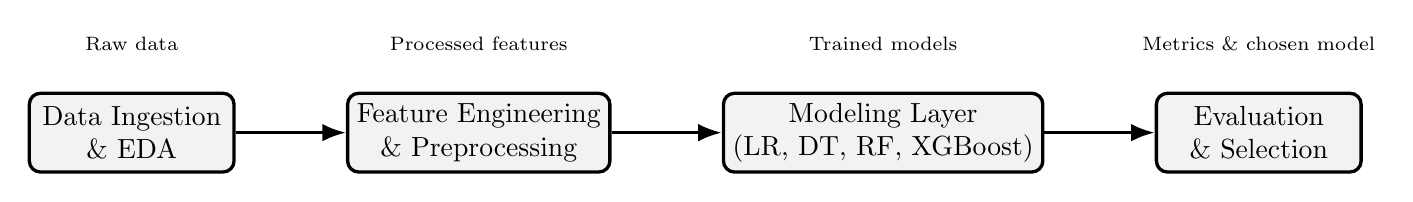
\begin{tikzpicture}[
        node distance = 1.4cm,
        box/.style = {
            rectangle,
            rounded corners,
            draw=black,
            very thick,
            minimum width=2.6cm,
            minimum height=1.0cm,
            align=center,
            fill=gray!10
        },
        arrow/.style = {
            -{Latex[length=3mm]},
            very thick
        }
    ]

    % Nodes
    \node[box] (data) {Data Ingestion\\\& EDA};
    \node[box, right=of data] (prep) {Feature Engineering\\\& Preprocessing};
    \node[box, right=of prep] (model) {Modeling Layer\\(LR, DT, RF, XGBoost)};
    \node[box, right=of model] (eval) {Evaluation\\\& Selection};

    % Arrows
    \draw[arrow] (data)  -- (prep);
    \draw[arrow] (prep)  -- (model);
    \draw[arrow] (model) -- (eval);

    % Shorter labels
    \node[above=0.4cm of data]  {\scriptsize Raw data};
    \node[above=0.4cm of prep]  {\scriptsize Processed features};
    \node[above=0.4cm of model] {\scriptsize Trained models};
    \node[above=0.4cm of eval]  {\scriptsize Metrics \& chosen model};

    \end{tikzpicture}%
    }
    \caption{Overall modeling pipeline for predicting online shoppers' purchasing intention.}
    \label{fig:pipeline}
\end{figure}


\subsection{Data Preprocessing}

\subsubsection{Exploratory Data Analysis}

Initial EDA revealed substantial class imbalance, with only 15.5\% of samples labeled as positive (\texttt{Revenue = 1}). Numerical features exhibited several high correlations (e.g., \textit{ProductRelated} and \textit{ProductRelated\_Duration}, $\rho > 0.90$). Categorical variables such as \textit{Month}, \textit{VisitorType}, and \textit{Region} required encoding.

\begin{figure}[H]
    \centering
    \includegraphics[width=\columnwidth]{correlation_heatmap.png}
    \caption{Correlation heatmap of numerical features.}
    \label{fig:correlation_heatmap}
\end{figure}

\subsubsection{Handling Missing Data}

The dataset contains no missing values; therefore, no imputation procedures were required.

\subsubsection{Feature Generation}

In addition to cleaning and encoding the raw attributes, we created two derived
features to capture additional behavioural patterns not explicitly represented
in the original dataset.

\paragraph{Total\_Time}
To aggregate a user's total engagement across different types of pages,
we summed the duration-based variables:

\begin{equation}
\begin{aligned}
\text{Total\_Time} &= \text{Administrative\_Duration} \\
                   &\quad + \text{Informational\_Duration} \\
                   &\quad + \text{ProductRelated\_Duration}
\end{aligned}
\end{equation}


This feature represents the overall time spent during a session and provides a
single continuous measure of user engagement intensity.

\paragraph{Is\_SpecialDay}
The original \texttt{SpecialDay} variable encodes proximity to a holiday using a
continuous value between 0 and 1. To simplify interpretability and model use,
we converted it into a binary indicator:

\begin{equation}
\text{Is\_SpecialDay} =
\begin{cases}
1, & \text{if SpecialDay} > 0 \\
0, & \text{otherwise}
\end{cases}
\end{equation}

This transformation distinguishes sessions that occur near significant holiday
periods, which often influence purchasing behaviour.

The inclusion of these two derived variables increased the dataset from 18 to 20
features and introduced higher-level representations that improved model
interpretability while preserving the underlying behavioural information.


\subsubsection{Feature Encoding}

Categorical variables were transformed using one-hot encoding:

\begin{lstlisting}
pd.get_dummies(df, columns=categorical_cols, drop_first=True)
\end{lstlisting}

Boolean variables (\textit{Weekend}, \textit{Revenue}) were encoded as 0/1.

\subsubsection{Feature Scaling}

Numerical variables were standardized using training-set statistics:

\begin{equation}
x_{\text{scaled}} = \frac{x - \mu_{\text{train}}}{\sigma_{\text{train}}}
\end{equation}

\begin{lstlisting}
scaler = StandardScaler()
X_train[num_cols] = scaler.fit_transform(X_train[num_cols])
X_test[num_cols]  = scaler.transform(X_test[num_cols])
\end{lstlisting}

Scaling ensures logistic regression behaves properly while maintaining consistent preprocessing across models.

\subsubsection{Feature Selection}

Two filter-based methods were applied:

\paragraph{Variance Threshold}
A threshold of 0.0 was used:
\begin{lstlisting}
VarianceThreshold(threshold=0.0)
\end{lstlisting}
And no features were removed.

\paragraph{Correlation-Based Filtering}
A pair of highly correlated features ($|\rho| \ge 0.90$) was identified, and one feature from the pair was removed to avoid redundancy.

\begin{table}[!ht]
\caption{Features Removed via Correlation Filtering ($|r| \ge 0.90$)}
\centering
\begin{tabular}{|l|c|}
\hline
\textbf{Feature Removed} & \textbf{Correlated With} \\ \hline
ExitRates & BounceRates ($r = 0.91$) \\ \hline
\end{tabular}
\label{tab:correlation_filtered}
\end{table}

\subsection{Algorithm Design}

We evaluated linear and nonlinear classifiers to compare interpretability and predictive power.

\subsubsection{Logistic Regression Models}

Three variants were trained:

\begin{itemize}
    \item \textbf{Baseline (No Penalty)}  
\begin{lstlisting}
LogisticRegression(penalty='none',
                   solver='lbfgs',
                   max_iter=2000)
\end{lstlisting}

    \item \textbf{Ridge (L2)}  
\begin{lstlisting}
LogisticRegression(penalty='l2',
                   C=0.01,
                   solver='lbfgs',
                   max_iter=2000)
\end{lstlisting}

    \item \textbf{LASSO (L1)}  
\begin{lstlisting}
LogisticRegression(penalty='l1',
                   C=0.1,
                   solver='liblinear',
                   max_iter=2000)
\end{lstlisting}
\end{itemize}

L1 regularization provided embedded feature selection, retaining 17 out of 38 features.

\subsubsection{Decision Tree Classifier}

A shallow decision tree (for interpretability) was tuned via GridSearchCV:

\begin{lstlisting}
DecisionTreeClassifier(criterion='entropy',
                       max_depth=4,
                       min_samples_split=2)
\end{lstlisting}

\subsubsection{Random Forest Classifier}

A Random Forest was tuned using ROC--AUC scoring:

\begin{lstlisting}
RandomForestClassifier(n_estimators=300,
                       max_depth=None,
                       min_samples_split=10,
                       class_weight='balanced',
                       random_state=42)
\end{lstlisting}

\subsubsection{XGBoost Classifier}

Boosted trees were tuned with:

\begin{lstlisting}
XGBClassifier(n_estimators=100,
              max_depth=3,
              learning_rate=0.1,
              subsample=1.0,
              colsample_bytree=1.0,
              eval_metric='logloss',
              random_state=42)
\end{lstlisting}

\subsection{Model Training}

All models were trained using the same protocol:

\begin{itemize}
    \item 70\% training, 15\% validation (via internal cross-validation), 15\% testing.
    \item Training performed with:
\begin{lstlisting}
model.fit(X_train, y_train)
\end{lstlisting}
    \item Predictions computed as:
\begin{lstlisting}
y_pred = model.predict(X_test)
y_proba = model.predict_proba(X_test)[:, 1]
\end{lstlisting}
    \item Evaluation metrics included Accuracy, Precision, Recall, F1-score, ROC--AUC, and PR--AUC.
\end{itemize}

This methodology ensures reproducibility and allows for direct comparison of linear and ensemble-based approaches under consistent preprocessing and evaluation criteria.

\begin{thebibliography}{99}

\bibitem{c1} Moro, S., Rita, P., and Cortez, P. (2016). "A Data-Driven Approach to Predict the Success of Bank Telemarketing." \textit{Decision Support Systems}, 62, 22–31.
\bibitem{c2} UCI Machine Learning Repository (2018). "Online Shoppers Purchasing Intention Dataset."
\bibitem{c3} Pedregosa, F. et al. (2011). "Scikit-learn: Machine Learning in Python." \textit{Journal of Machine Learning Research}, 12, 2825–2830.
\bibitem{c4} Powers, D. M. W. (2011). "Evaluation: From Precision, Recall and F-measure to ROC, Informedness, Markedness and Correlation." \textit{Journal of Machine Learning Technologies}, 2(1), 37–63.
\bibitem{c5} Baati, K., \& Mohsil, M. (2020). Real-Time Prediction of Online Shoppers’ Purchasing Intention Using Random Forest. Artificial Intelligence Applications and Innovations: 16th IFIP WG 12.5 International Conference, AIAI 2020, Neos Marmaras, Greece, June 5–7, 2020, Proceedings, Part I, 583, 43–51. https://doi.org/10.1007/978-3-030-49161-1\_4

\end{thebibliography}

\end{document}
